\documentclass[10pt]{article}
\usepackage[OE]{express}

\begin{document}
\title{Determining Single-Molecule Orientation With Polarized Illumination:
  Instrument Design and Forward Model}

\author{Talon Chandler,\authormark{1} Author Two,\authormark{2,*} and Author Three\authormark{2,3}}

\address{\authormark{1}Peer Review, Publications Department, The Optical Society, 2010 Massachusetts Avenue NW, Washington, DC 20036, USA\\
\authormark{2}Publications Department, The Optical Society, 2010 Massachusetts Avenue NW, Washington, DC 20036, USA\\
\authormark{3}Currently with the Department of Electronic Journals, The Optical Society, 2010 Massachusetts Avenue NW, Washington, DC 20036, USA}

\email{talonchandler@talonchandler.com} %% email address is required

%%%%%%%%%%%%%%%%%%% abstract and OCIS codes %%%%%%%%%%%%%%%%
\begin{abstract*}
Abstract here. 
\end{abstract*}

\ocis{(180.0180) Microscopy; (260.5430) Polarization; (110.0110) Imaging systems; (180.2520) Fluorescence microscopy; (180.6900) Three-dimensional microscopy.}  

%%%%%%%%%%%%%%%%%%%%%%% References %%%%%%%%%%%%%%%%%%%%%%%%%
\begin{thebibliography}{99}
\bibitem{gallo99} K. Gallo and G. Assanto, ``All-optical diode based on second-harmonic generation in an asymmetric waveguide,'' \josab {\bfseries 16}(2), 267--269 (1999).
\end{thebibliography}

\section{Introduction}

\section{Methods}
Illumination forward model, CRLB, dispersion index

\section{Results}
\subsection{One-Arm Designs}
\begin{figure}[htbp]
\centering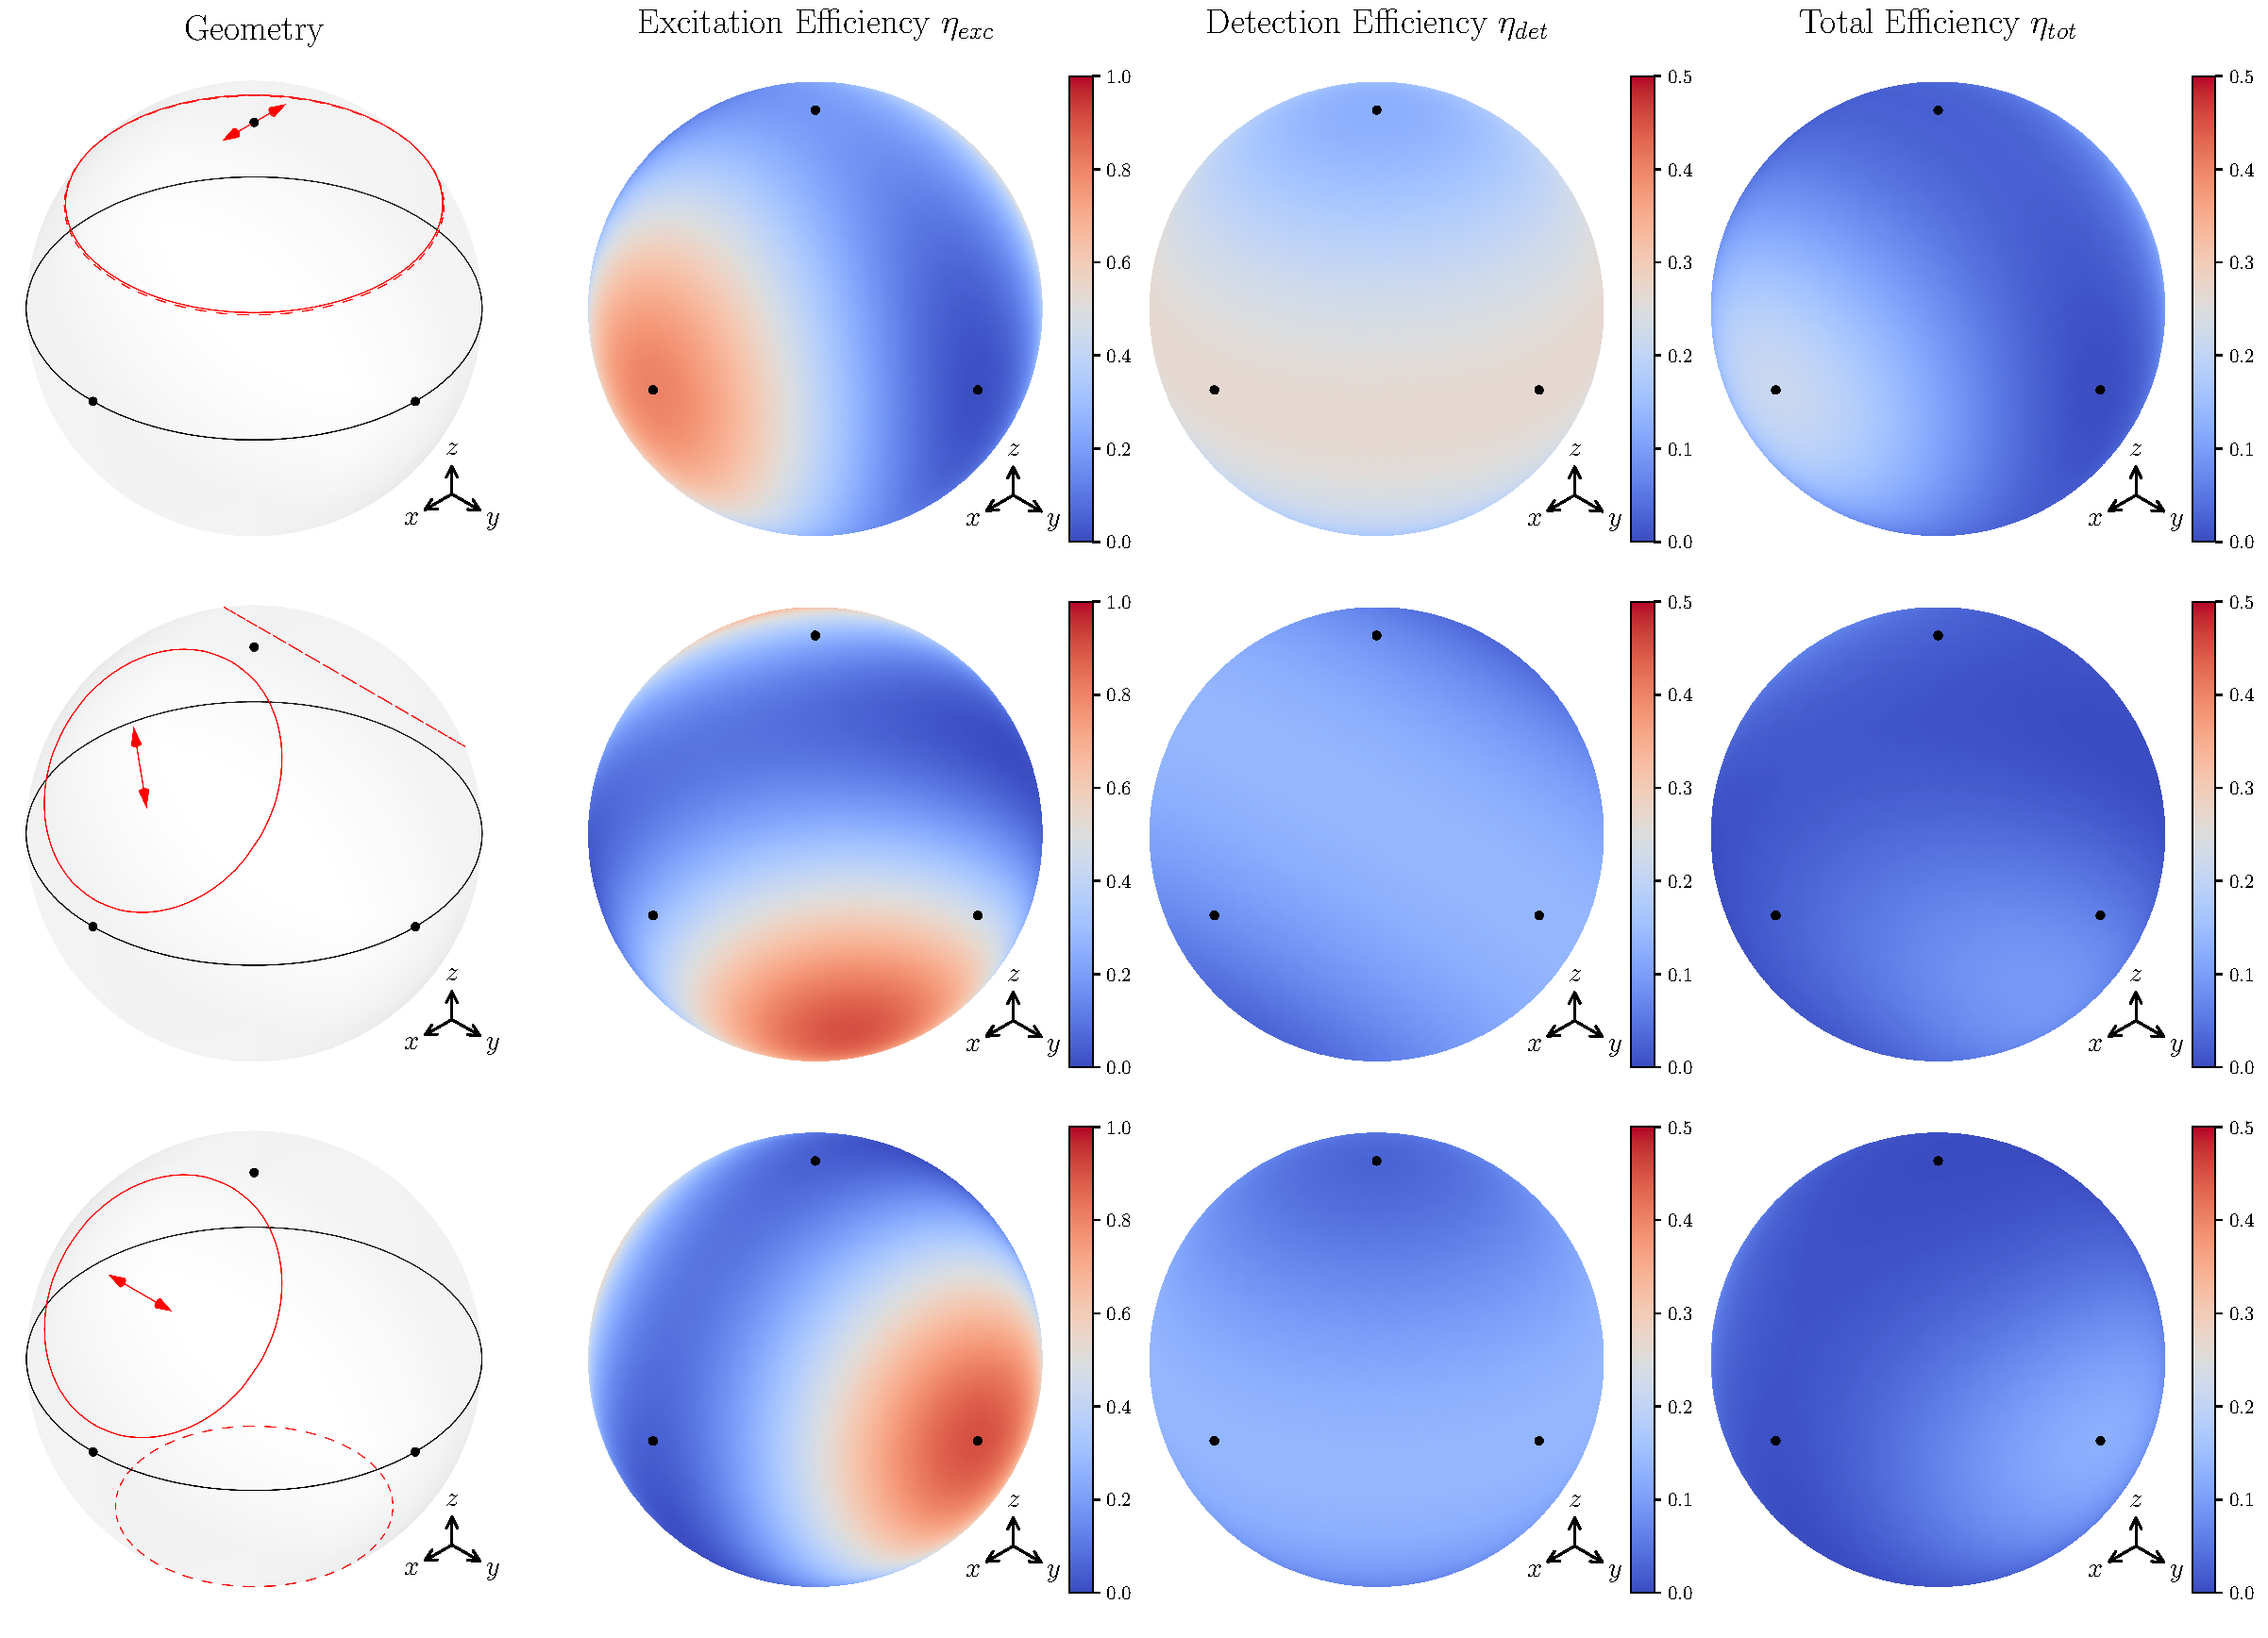
\includegraphics[width=\textwidth]{single-frame}
\caption{Caption 123}
\end{figure}

\subsection{Two-Arm Designs}
\subsection{Three-Arm Designs}

\section{Discussion}

\section{Conclusion}
After proofreading the manuscript, compress your .TEX manuscript file and all
figures (which should be in EPS format, or PDF format if you are using
PDF-\LaTeX) in a ZIP, TAR or TAR-GZIP package. Prism, OSA's article tracking
system, will process in \LaTeX mode by default but will use PDF-\LaTeX if PDF
figure files are detected. Note: TAR or TAR-GZIP is no longer required. All
files must be referenced at the root level (e.g., file \texttt{figure-1.eps},
not \texttt{/myfigs/figure-1.eps}). If there is video or other multimedia, the
associated files should be uploaded separately.

\section*{Funding}
TODO

\section*{Acknowledgments}
TODO

\section*{Disclosures}
The authors declare that there are no conflicts of interest related to this article.

\end{document}
